\chapter{费米子符号与超对称相消}

\lectureoverview{超对称将玻色子与费米子联系起来，但在写下其代数之前，更容易看清为何需要这样一种关系。我们从旋转的拓扑开始，通过干涉使费米子波函数的符号成为可观测的，从交换反对称性导出闭合费米子圈的负号，然后利用玻色圈与费米圈相反的符号来引出真空能和标量自能的相消。后半部分追问超对称可以被破坏到何种程度、人们如何探测超对称伙伴粒子，以及为什么精确的超对称会抹去普通的原子壳层结构。}

\section{超对称之前：旋转的一个奇特之处}

超对称是费米子与玻色子之间的一种对称性。然而，在尝试构造它之前，值得回顾一下这两类粒子对旋转的响应有多么不同。这个问题本身始于一个拓扑事实，它容易演示，而一旦见过就出奇地难以忘记。

将一只手手掌朝上，转动手腕\(2\pi\)。手回到了原来的朝向，但手臂显然并未回到一个等价的构型：它被扭转了。继续再转\(2\pi\)，必要时让手臂随之移动，扭转便可消除。因此，在周围环境保持固定时，\(2\pi\)旋转不能连续地形变到无旋转，而\(4\pi\)旋转则可以。这个手的演示是最字面意义上的“挥手证明”。

不依赖解剖结构也能说明同一点。把一个小球放在固定的盒子里，用任意多根柔韧、可拉伸但不可断裂的绳子把小球系到壁上。将小球旋转一次，转过\(2\pi\)。绳子变得缠结，仅靠绳子自身的运动无法恢复原来的构型。将小球总共转过\(4\pi\)，绳子便可绕过小球移动，直到缠结消失。壁代表空间无穷远：这一比较之所以有意义，只是因为边界并未随小球一起旋转。

\begin{classroomqa}
\audiencequestion{能否通过旋转盒子来消除缠结？\lecturetimestamp{00:02:53}}
\lecturerresponse{那会改变问题。盒子代表空间无穷远，是保持固定的。我们比较的是物体相对于其周围环境的旋转，而不是物体与周围环境的共同旋转。}
\end{classroomqa}

\begin{classroomqa}
\audiencequestion{为什么不干脆把小球再旋转\(2\pi\)？\lecturetimestamp{00:03:20}}
\lecturerresponse{这正是区分两种情形之处。不再进一步旋转小球，一次\(2\pi\)旋转留下的缠结无法消除。在第二次旋转之后，总共达到\(4\pi\)，它就可以消除。}
\end{classroomqa}

用现代群论语言来说，旋转群有两类拓扑上不同的闭合路径：
\begin{equation}
\pi_1\!\left(SO(3)\right)\cong \mathbb Z_2.
\end{equation}
单次遍历是非平凡的，但遍历两次给出平凡类。
等价地，\(SU(2)\)是\(SO(3)\)的双重覆盖。这就是费米子符号的几何前史。

\editorialnote{\(SO(3)\)、\(SU(2)\)以及基本群的语言使拓扑变得明确。手臂演示和绳子演示在几何上确立了同样的二值行为。}

\section{\texorpdfstring{\(2\pi\)}{2 pi}旋转对量子态的作用}

现在固定一个粒子的位置，只保留其自旋态，记为\(\ket{\psi}\)。整数自旋粒子是玻色子，半整数自旋粒子是费米子。物理旋转可以通过将带电自旋置于强磁场中并旋转磁场来实现，或者让自旋在固定磁场中进动所需的角度。

\begin{classroomqa}
\audiencequestion{在实验室中，电子自旋究竟如何才能真正被旋转？\lecturetimestamp{00:05:26}}
\lecturerresponse{磁场提供了把手。人们可以旋转足够强的磁场，使自旋跟随它，或者让自旋绕固定磁场进动。用手抓住电子并不是一种有竞争力的实验方法。}
\end{classroomqa}

假设完整旋转\(2\pi\)使态乘以一个相位：
\begin{equation}
R(2\pi)\ket{\psi}=\xi\ket{\psi}.
\end{equation}
将该操作执行两次得到
\begin{equation}
R(4\pi)\ket{\psi}=\xi^2\ket{\psi}.
\end{equation}
由于\(4\pi\)路径在拓扑上是平凡的，在这一比较中它必须表现为恒等操作。因此
\begin{equation}
\xi^2=1,
\qquad
\xi=+1\ \hbox{or}\ -1.
\end{equation}
玻色子实现正号，费米子实现负号：
\begin{align}
R(2\pi)\ket{\psi_B}&=+\ket{\psi_B},\\
R(2\pi)\ket{\psi_F}&=-\ket{\psi_F}.
\end{align}
对于具有确定自旋\(j\)的态，简洁的表述是
\begin{equation}
R(2\pi)=(-1)^{2j}.
\end{equation}
文字记录简要地说第二种可能性是乘以\(2\pi\)；周围的推导和板书论证表明，所意图的因子是\(-1\)。

起初这似乎没有物理意义。如果整个波函数改变符号，
\begin{equation}
\Psi\longmapsto-\Psi,
\end{equation}
那么概率不变，因为
\begin{equation}
(-\Psi)^*(-\Psi)=\Psi^*\Psi.
\end{equation}
取两群制备相同的电子，将其中一群的每个成员旋转 \(2\pi\)，另一群保持不变。对孤立成员的任何测量都无法揭示它来自哪一群。整体相位不是可观测量。

\section{使负号成为相对的}

当符号被施加于波函数的一个相干分支而不施加于另一个分支时，它就变得可观测了。让电子逐个通过双路径装置。不要确定走的是哪条路径，因为路径信息会破坏干涉。设上、下振幅分别为 \(\psi_1\) 和 \(\psi_2\)，于是重新组合后的态为
\begin{equation}
\Psi=\psi_1+\psi_2.
\end{equation}
想象暂时将每个分支困在各自的磁场区域中。只将与第二个分支相关的磁场旋转 \(2\pi\)。如果粒子是费米子，态变为
\begin{equation}
\Psi'=\psi_1-\psi_2.
\end{equation}
这不再是一个整体符号。相对相位将干涉极大变为极小。如果两个返回的波包关于探测器中心互为镜像，则反对称组合在中心处为零：
\begin{equation}
\Psi'(0)=\psi_1(0)-\psi_2(0)=0.
\end{equation}
因此电子永远不会在该对称点被探测到。若改为旋转两个分支，则会产生 \(-\psi_1-\psi_2=-\Psi\)，这没有可观测效应。

讲座强调了该实验的关系性本质。将一个磁场区域相对于另一个旋转，类似于让球旋转而盒子保持固定。将两个区域一起旋转，则类似于让球和盒子一起旋转。相对 \(4\pi\) 旋转会消除该效应，因为此时费米子态以正号返回。该实验由 Yakir Aharonov 和 Leonard Susskind 于 1967 年提出，后来以干涉测量形式实现，讲座中顺带提到了这一点。同样的原理可应用于电子或带电离子：移动的条纹图样标识半整数自旋态，而未移动的图样标识整数自旋态。

\begin{classroomqa}
\audiencequestion{如果相对磁场旋转 \(4\pi\)，移动的图样会回到原来的图样吗？\lecturetimestamp{00:12:21}}
\lecturerresponse{会。两次符号变化相乘为 \(+1\)，因此导致极大与极小互换的相对相位消失了。}
\end{classroomqa}

\begin{classroomqa}
\audiencequestion{盒子中的绳子应当在多大程度上被字面地关联到费米子？\lecturetimestamp{00:13:43}}
\lecturerresponse{它们是一种拓扑助记，并非附着在电子上的物理绳子。玻色子的行为就好像 \(2\pi\) 旋转没有留下记忆；费米子则精确地保留由非平凡缠绕所表示的符号记忆。}
\end{classroomqa}

\begin{classroomqa}
\audiencequestion{两个磁场区域中有两个电子吗，一个被旋转而另一个没有？\lecturetimestamp{00:14:29}}
\lecturerresponse{没有。只有一个处于相干空间叠加态的电子。它有占据任一分支的振幅，而装置不得揭示它占据了哪个分支。旋转一个区域会改变一个振幅相对于另一个振幅；旋转两者只改变共同相位。}
\end{classroomqa}

角度 \(2\pi\) 很特殊，因为自旋取向回到自身，而旋量获得一个符号。一般的相对旋转也会改变自旋取向。如果两个路径态返回时自旋态分别为 \(\ket{\chi_1}\) 和 \(\ket{\chi_2}\)，则干涉项正比于
\begin{equation}
\braket{\chi_1}{\chi_2}.
\end{equation}
其大小控制条纹可见度。\editorialnote{自旋重叠公式是对讲座中关于干涉部分损失和完全损失的定性讨论的标准补充。} 正交自旋态携带完美的路径信息，不发生干涉。

\begin{classroomqa}
\audiencequestion{如果测量电子位于哪个磁场区域，会发生什么？\lecturetimestamp{00:18:03}}
\lecturerresponse{干涉图样被破坏。任何区分两条路径的记录都会消除其振幅的相干叠加。}
\end{classroomqa}

\begin{classroomqa}
\audiencequestion{如果所有自旋都从同一方向开始，并且最终测量自旋，那么 \(2\pi\) 操作本身会改变该方向吗？\lecturetimestamp{00:18:17}}
\lecturerresponse{不会。经过 \(2\pi\) 之后，物理自旋方向相同；只有费米子分支获得了一个负号。这就是为什么该操作能够改变干涉，而不会留下不同的自旋取向作为路径标记。}
\end{classroomqa}

\begin{classroomqa}
\audiencequestion{如果场只转过\(\pi\)，而不是\(2\pi\)，会怎样？\lecturetimestamp{00:18:43}}
\lecturerresponse{那么自旋方向就会改变。上自旋分支和下自旋分支是可区分的，因而不能干涉。中间角度会连续地降低可见度；相对转过\(180^\circ\)会将其完全破坏。}
\end{classroomqa}

\section{交换对称性与闭合圈的符号}

关于旋转的讨论已经分离出一个费米子负号。当全同粒子交换时，会出现第二个密切相关的符号。对于双粒子波函数，
\begin{align}
P_{12}\Psi_B(1,2)&=+\Psi_B(1,2)=+\Psi_B(2,1),\\
P_{12}\Psi_F(1,2)&=-\Psi_F(1,2)=-\Psi_F(2,1).
\end{align}
玻色子态是对称的，费米子态是反对称的。

\begin{figure}[htbp]
\centering
\includegraphics[width=0.74\textwidth]{lecture_02_figure_02.png}
\lectureframe{00:24:27}
\caption{用态记号表示的交换论证。画面中只有 ket 标签是可靠可辨的；反对称性方程是正文中打出的，而不是归因于被遮挡的板书。}
\end{figure}

现在，我们无需计算积分，就可以确定闭合粒子圈的相对符号。考虑一个没有外腿的真空费曼图。它可以被想象为一个粒子在时空中描出一条闭合路径，或者被想象为一对粒子-反粒子被产生、随后又被湮灭。这样的真空图对真空振幅有贡献，因而对真空能量有贡献。

从两个互不连通的圈副本开始。不连通图相乘，因此如果一个圈的符号是\(\sigma\)，那么这一对的符号就是
\begin{equation}
\sigma^2=+1.
\end{equation}
在共同时刻，比如\(t=0\)，把两个圈都切开。在该时间切片上有两个全同粒子。不交换它们而重新连接，两个分离的圈就回来了。在重新连接之前交换这两个粒子，拓扑就变成一个圈。交换对玻色子贡献\(+1\)，对费米子贡献\(-1\)。由于起始的双圈符号为正，所得的单圈符号为
\begin{equation}
\begin{aligned}
\operatorname{sign}(\text{closed boson loop})&=+1,\\
\operatorname{sign}(\text{closed fermion loop})&=-1.
\end{aligned}
\end{equation}
更一般地，一个含有\(L_F\)个独立闭合费米子圈的图带有因子
\begin{equation}
(-1)^{L_F}.
\end{equation}
本讲有意从交换而不是通过调用格拉斯曼积分来推导这条规则。这个初等论证使该符号的物理起源变得可见。

\section{相反的圈符号与真空能量}

玻色子真空圈以一种符号提高真空贡献，而费米子圈以相反的符号进入。这立刻给人以启发，因为观测到的暗能量密度与量子场论中朴素的截断估计相比极其微小。本讲把这一臭名昭著的不符引用为大约\(123\)个数量级。精确的指数取决于使用哪个紫外标度；持久不变的一点是这种惊人的不匹配。

一个圈的值不仅取决于统计性质。它还取决于质量、电荷、多重数和相互作用。然而，如果一个玻色子和一个费米子在所有相关性质上都匹配，它们等大的贡献就可以相消：
\begin{equation}
\begin{gathered}
m_B=m_F,\qquad q_B=q_F,\qquad g_B=g_F,\\
\Delta\rho_{\mathrm{vac}}^{(B)}
+\Delta\rho_{\mathrm{vac}}^{(F)}=0.
\end{gathered}
\end{equation}
这一观察并没有解决宇宙学常数问题。它只是提供了仅靠普通玻色子圈无法提供的东西：相反符号的贡献。在一个严格未破缺的全局超对称理论中，在适当假设下，真空能相消确实可以是精确的；超对称破缺之后，观测到的微小非零值仍然无法解释。\editorialnote{这一限定把本讲的动机与困难得多的宇宙学常数问题区分开来。}

人们已经知道，精确匹配并不能描述自然。如果电子有一个质量相同、电荷相同的自旋为零的伙伴，那么电子-正电子通过虚光子湮灭就可以产生一对这样的粒子：
\begin{equation}
e^-e^+\longrightarrow\gamma^*
\longrightarrow\widetilde e^-\widetilde e^+.
\end{equation}
一个简并的带电标量粒子不可能逃过普通的对撞机实验。因此，玻色子-费米子反射不可能是观测到的谱的精确对称性。这是粒子类型上的反射，而不是物理空间中的反射。

\section{更直接的目标：标量自能}

真空能量是第一个例证，但本讲主要关心的是标量质量的辐射不稳定性。一个裸质量起初为零的标量粒子可以接收到一个对截断二次敏感的修正。示意性地，
\begin{equation}
\Delta m_H^2\sim \frac{g_B^2}{16\pi^2}\Lambda^2
\end{equation}
来自一个玻色子圈。费米子质量有一种不同的保护：当一个无质量费米子具有精确的手征对称性时，辐射修正不能产生加性质量项。那就是上一讲中的左右论证。

现在想象一种足够严格的对称性，它能把一个标量和一个费米子放进同一个多重态，并使它们的相互作用相匹配。于是费米子圈以相反的符号出现：
\begin{equation}
\Delta m_H^2
\sim
\frac{g_B^2-g_F^2}{16\pi^2}\Lambda^2+\cdots .
\end{equation}
如果超对称强制要求\(g_B=g_F\)且质量相等，那么二次项就会抵消。费米子所受到的这种保护由此传递给了它的玻色子伙伴。这不仅仅是两个图之间的数值巧合；对称性必须在每一阶以及每一种允许的相互作用中强制实现这种抵消。

这块大范围的黑板对比表明，讲座正从孤立的圈图转向传播粒子的成对圈图修正。

\begin{figure}[htbp]
\centering
\includegraphics[width=0.79\textwidth]{lecture_02_figure_04.png}
\lectureframe{00:40:23}

\medskip
\begin{tikzpicture}[scale=0.9]
\draw (-4.2,0) circle (0.55);
\draw[dashed] (-2.4,0) circle (0.55);
\draw (0,0) -- (3.7,0);
\fill (1.85,0) circle (0.055);
\draw (1.85,0) -- (1.85,0.25);
\draw[dashed] (1.85,0.85) circle (0.6);
\end{tikzpicture}
\caption{普通圈图与伙伴圈图拓扑结构的整板对比。这份打字草图只保留了可见的拓扑对比；它并未标出被遮挡的粒子标签。}
\end{figure}

课间休息之后，论证从所谓的零阶图像重新开始。这并不是微扰论中的某一阶。它指的是最粗略但仍有用的描述：
\begin{quote}
每一种粒子都有一个统计性质相反的超级伙伴。每个费米子都有一个玻色子伙伴，每个玻色子都有一个费米子伙伴。
\end{quote}
在一个严格的超对称理论中，这些伙伴还会是简并的，也就是说质量相等。自然界并非以这种方式简并。不过，如果质量不相等但相差不太远，抵消仍可能足够好，从而防止标量修正爆炸性地变大。在软超对称破缺下，危险能标被示意性地替换为超级伙伴的质量劈裂：
\begin{equation}
\Delta m_H^2\sim
\frac{g^2}{16\pi^2}\,\Delta m_{\mathrm{SUSY}}^2
\ln\!\frac{\Lambda^2}{\Delta m_{\mathrm{SUSY}}^2}
\end{equation}
直到依赖于模型的系数。\editorialnote{这个公式表达了讲座的定性陈述：不完美的质量匹配会留下一个由劈裂控制的残余修正；它并非从黑板上抄录而来。}

\section{破缺的超对称性与2010实验赌注}

在2010年录制这场讲座时，尚未观测到任何超级伙伴。直接的推论是：这些伙伴如果真实存在，必定比已知粒子更重，也必定超出更早机器的探测范围。超对称模型还区分那些只有在电弱对称性破缺之后才获得质量的粒子，与那些被允许携带更大的保持对称性的质量的态。讲座以此作为理由，说明为什么超对称谱中可见的那一半可能较轻，而未被看见的那一半更重，同时坦率地称这种安排有些牵强。Susskind陈述了他自己的预期，即超级伙伴会被探测到，但随即将其标记为猜测而非结果。

因此，大型强子对撞机在这场讲座的展望中处于核心地位。人们期望它既搜寻希格斯玻色子，也搜寻超级伙伴。这些陈述必须放在2010年的背景下来读：讲座是在希格斯发现之前、也是在后来LHC搜寻结果之前，解释这一实验赌注。

为什么一个由自然性驱动的超级伙伴不应位于普朗克能标？因为那样它就无法完成分配给它的任务。如果玻色子和费米子的质量相差极大，它们的圈积分在较轻质量以上就不再抵消。残余的标量修正大致由重的劈裂而非弱能标决定。处在任意遥远能标上的超对称仍然是一种数学对称性，但它不再能为轻的希格斯部门提供有说服力的解释。

讲座将此转化为其时代的预期：相关的劈裂应大致在几百GeV之内，因而处于LHC的探测范围之内。这个数值估计是历史性的且依赖于模型；逻辑链条更为重要：
\begin{equation}
\begin{gathered}
\text{Higgs protection}\\
\Downarrow\\
\text{effective boson--fermion cancellation}\\
\Downarrow\\
\Delta m_{\mathrm{SUSY}}\ \text{not too large}.
\end{gathered}
\end{equation}

\begin{classroomqa}
\audiencequestion{所有费米子贡献是否可能只是在总体上抵消所有玻色子贡献，而不需要一一对应的伙伴？\lecturetimestamp{00:45:01}}
\lecturerresponse{它们在数值上可以抵消，但那将是一种偶然的抵消，其精细调节程度与最初的问题一样。超对称的提议更强：合理的假设强制贡献相匹配，而破缺的超对称则解释了为什么质量只是近似匹配。真空能是那个例证；这里直接关心的是希格斯自能。}
\end{classroomqa}

\begin{classroomqa}
\audiencequestion{把一种总体相消称为不自然，是否已经预设了一种还原论式的理论组织方式？\lecturetimestamp{00:47:51}}
\lecturerresponse{这是一个合理的质疑。没有人对自然性有最终的定义，而这种探索在一定程度上就是在摸索一个令人信服的解释。超对称性和自发超对称破缺提供了已知的数学框架，能够强制实现所期望的模式。尚未解决的问题是，自然界是否采用这一框架，以及它是否唯一。}
\end{classroomqa}

\section{直接产生、虚效应与衰变链}

一个重粒子不必在壳产生就能影响实验。它可以在一个圈图内部以虚粒子的方式出现，并轻微改变普通的电子-正电子散射振幅。因此，即使质心能量低于直接对产生的阈值，精确的电弱测量也会对超伴侣施加限制
\begin{equation}
\sqrt{s}<2m_{\widetilde p}.
\end{equation}
讲座在2010年的评估是，精确数据已经在挤压超对称参数空间，但尚未将其排除。

\begin{classroomqa}
\audiencequestion{能否像早先的重粒子在直接观测之前通过精确的产生率受到限制那样，间接推断出超伴侣？\lecturetimestamp{00:49:01}}
\lecturerresponse{可以。一个虚超伴侣圈图会轻微改变普通振幅，因此问题就变成了高精度电弱现象学，而不是直接产生。一台干净且能量足够高的电子-正电子对撞机会特别有用。质子碰撞则更为杂乱，因为质子是夸克和胶子的复合态；人们实际上是在让涨落的组分相互碰撞，而不是两个初始条件精确已知的基本粒子。}
\end{classroomqa}

一名学生问及反向运行该反应，即从大量超粒子开始。障碍不在于时间反演对称性，而在于可获得性。重超伴侣必须首先被产生出来，而其中大多数预计会迅速衰变为更轻的态。

\begin{classroomqa}
\audiencequestion{如果一个宇宙中包含许多超粒子，其中两个能否碰撞并转变为普通粒子？\lecturetimestamp{00:53:43}}
\lecturerresponse{原则上，相关反应存在逆通道，但重超伴侣预计不会保持自由地大量存在。它们会衰变到更低能量的态，因此实验必须首先提供足够的碰撞能量来产生它们。}
\end{classroomqa}

这就引出了暗物质问题。在许多超对称模型中，一条离散的选择定则阻止衰变链中最后一个超伴侣完全消失。于是每个较重的超伴侣都级联衰变到最轻超伴侣，即LSP。如果LSP是电中性的，它就可以稳定且难以探测，从而成为可能的暗物质候选者。文字记录在这一段对话中曾有一次说成“暗能量”，但听众的问题和粒子描述无疑涉及的是暗物质。

\begin{classroomqa}
\audiencequestion{超伴侣的快速衰变是否与某个超伴侣可能构成暗物质的提议相冲突？\lecturetimestamp{00:54:53}}
\lecturerresponse{不冲突。在要求每条衰变链末端都有一个超伴侣的模型中，大多数超伴侣可以衰变，而最轻的那个保持稳定。电荷通常会带来额外的现象学困难，因此可行的LSP很可能是中性的。它原则上并非不可探测，但它不会留下带电超电子那种明显的电离径迹。}
\end{classroomqa}

\section{匹配意味着匹配耦合}

仅靠质量匹配是不够的。比较一个电子真空圈图和一个超电子圈图。它们相反的统计性质给出相反的符号，但要使大小相等，就要求质量相等。现在接上两个外线光子。系数中还包含电耦合，因此相消要求电荷相等：
\begin{equation}
\begin{gathered}
q_{\widetilde e}=q_e,\\
\mathcal A_{\mathrm{loop}}^{(e)}
+\mathcal A_{\mathrm{loop}}^{(\widetilde e)}=0,\\
\text{provided the full couplings match.}
\end{gathered}
\end{equation}
在任何层面上出现不匹配，都会留下一个未被相消的发散项。超对称性之所以有价值，是因为它不仅关联名称和自旋，还关联相互作用。

\begin{figure}[H]
\centering
\includegraphics[width=0.66\textwidth]{lecture_02_figure_05.png}
\lectureframe{00:57:15}

\medskip
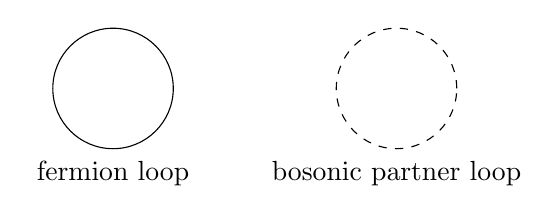
\begin{tikzpicture}[scale=0.9]
\draw (-2.0,0) circle (0.85);
\draw[dashed] (2.0,0) circle (0.85);
\node at (-2.0,-1.2) {fermion loop};
\node at (2.0,-1.2) {bosonic partner loop};
\end{tikzpicture}
\caption{在电荷匹配论证中比较的实线和虚线圈图。被裁掉的外线标记未被重建，因为仅凭这一帧无法确定每一处连接。}
\end{figure}

\begin{classroomqa}
\audiencequestion{超伴侣之所以未被探测到，是否可能仅仅因为它们的耦合常数不同？\lecturetimestamp{00:56:23}}
\lecturerresponse{如果要求同样的图相消，那就不可能。加入光子相互作用会检验每条线的电荷。不相等的耦合给出不相等的数值圈因子，并恢复出很大的剩余项。对称性必须匹配相应的电荷和相互作用。}
\end{classroomqa}

\begin{classroomqa}
\audiencequestion{光子的超对称伴子也应当是无质量的吗？\lecturetimestamp{00:58:01}}
\lecturerresponse{在严格的超对称理论中，它会是无质量的，因为它会与光子简并。观测到的世界并非严格超对称，因此物理的光微子样态不必与光子具有相同的质量。}
\end{classroomqa}

\section{超对称伴子词典}

这些命名规则并不优雅，但很实用。玻色子获得一个费米子伴子，其名称常以\emph{-ino}结尾：光子与光微子、\(W\)与wino、\(Z\)与zino、胶子与胶微子、希格斯与希格斯微子、引力子与引力微子。普通费米子获得一个玻色子伴子，其名称通常以\emph{s-}开头：电子与超电子、夸克与超夸克。

\begin{center}
\begin{tabular}{@{}>{\raggedright\arraybackslash}p{0.40\linewidth}>{\raggedright\arraybackslash}p{0.52\linewidth}@{}}
\toprule
普通态 & 超对称伴子与自旋变化\\
\midrule
标量希格斯，\(j=0\) & 希格斯微子，\(j=\tfrac12\)；\(\Delta j=+\tfrac12\)\\
规范玻色子，\(j=1\) & 规范微子，\(j=\tfrac12\)；\(\Delta j=-\tfrac12\)\\
物质费米子，\(j=\tfrac12\) & 超费米子，\(j=0\)；\(\Delta j=-\tfrac12\)\\
引力子，\(j=2\) & 引力微子，\(j=\tfrac32\)；\(\Delta j=-\tfrac12\)\\
\bottomrule
\end{tabular}
\end{center}

一般关系是，同一超多重态中的成员相差半个单位的自旋：
\begin{equation}
\Delta j=\frac12.
\end{equation}
讲义中的粗略例子将自旋为\(\tfrac12\)的物质费米子与标量配对，将自旋为1的规范玻色子与自旋为\(\tfrac12\)的规范微子配对。一个完整的相互作用模型在对称性破缺后可以使各态混合，因此物理的质量本征态不必保留这些最简单的名称。

\begin{classroomqa}
\audiencequestion{所有新的标量伴子是否都可能经历它们自身的自发对称性破缺？\lecturetimestamp{01:01:27}}
\lecturerresponse{标量场可以获得期望值，但任意额外的对称性破缺在现象学上将是灾难性的。一个可行的超对称模型必须安排其标量势，使得色、电荷以及其他所需对称性不会以错误的方式被破缺。}
\end{classroomqa}

\begin{classroomqa}
\audiencequestion{希格斯微子是否具有对应于希格斯四重项的特殊相互作用？\lecturetimestamp{01:02:19}}
\lecturerresponse{超对称不仅匹配粒子，也匹配相互作用。这一关系并非通过天真地将每条希格斯线替换为希格斯微子线而得到，但标量四重项以及相关的费米子和辅助场相互作用属于同一个受约束的结构。这些细节在讲义中尚未展开。}
\end{classroomqa}

\begin{classroomqa}
\audiencequestion{\(2\pi\)对\(4\pi\)的旋转定理在其他维度中是否有类似物？\lecturetimestamp{01:03:07}}
\lecturerresponse{有，但维度会改变可能性。在二维空间中，交换路径可以相互缠绕，从而允许任意子，其交换相位比玻色子的\(+1\)和费米子的\(-1\)更为一般。这类激发出现在凝聚态系统中，但它们不在本课程的路线之内。}
\end{classroomqa}

\section{为什么严格的超对称会抹除化学}

我们最后问，一个严格超对称的世界会是什么样子。这里的严格意味着每一对粒子-超对称伴子都具有相等的质量和匹配的相互作用。电子会有一个玻色性的超电子，具有相同的质量和电荷，而无质量的光子会有一个无质量的费米性光微子：
\begin{equation}
m_{\widetilde e}=m_e,
\qquad
q_{\widetilde e}=q_e,
\qquad
m_{\widetilde\gamma}=m_\gamma=0.
\end{equation}

化学中熟悉的周期结构依赖于费米统计。氢在其最低轨道上有一个电子。氦在那里容纳两个电子，因为自旋标记不同。锂的第三个电子必须占据更高的轨道：泡利不相容原理阻止三个全同电子占据同一个单粒子态。那个外层电子具有更多能量，并倾向于向内掉落，通常会发射一个光子，但已填满的低能态阻止了这一跃迁。

严格的超对称打开了另一条通道：
\begin{equation}
e^-_{\mathrm{outer}}
\longrightarrow
\widetilde e^-_{\mathrm{inner}}
+
\widetilde\gamma .
\end{equation}
初始电子和发射出的光微子是费米子，而剩余的超电子是玻色子。因为超电子服从玻色统计而非费米统计，最终的超电子不会被排除在已被占据的低轨道之外。因此，价电子可以转换并向内掉落。

\begin{figure}[H]
\centering
\includegraphics[width=0.62\textwidth]{lecture_02_figure_06.png}
\lectureframe{01:09:18}

\medskip
\begin{tikzpicture}[scale=0.9]
\fill (0,0) circle (0.075);
\draw (0,0) circle (0.72);
\draw (0,0) circle (1.45);
\draw[-{Latex[length=2.2mm]}] (1.42,0.2) .. controls (1.2,0.52) and (0.92,0.42) .. (0.72,0.1);
\draw[decorate,decoration={snake,amplitude=1.4pt,segment length=7pt},-{Latex[length=2.2mm]}]
  (1.58,0) -- (3.55,0);
\node[above] at (2.7,0.12) {$\widetilde\gamma$};
\node[below] at (0,-1.65) {selectron drops to a lower orbital};
\end{tikzpicture}
\caption{用于说明为什么严格的超对称会改变化学的原子跃迁。向外传播的波浪线是可见的；将其认定为光微子来自文字记录。}
\end{figure}

这一点并不局限于类锂原子。在大原子中，正是价电子造就了化学的多样性。如果它们能够反复转化为玻色性的超电子，它们就可以挤入能量上可用的最低区域，而不是填充壳层。其结果将类似于原子核附近聚集的玻色子布居，而不是我们熟悉的价轨道结构。由方向性键和部分填充壳层构成的分子将无法以可辨认的形式存在。讲座把这种假想的锂的后代称为\emph{slithium}，但这个玩笑带有一个严肃的结论：精确的超对称性会产生不同于普通化学、因而也不同于普通生物学的物质。

\begin{classroomqa}
\audiencequestion{电子到超电子的跃迁会不会耦合得如此之弱，以至于普通原子能够存活下来？\lecturetimestamp{01:10:23}}
\lecturerresponse{在正在设想的精确理论中不会。超对称性把这种跃迁与电磁相互作用联系起来，因此它的耦合由电荷固定，而不是可以自由选择得极其微小。讲座给出类锂原子的粗略寿命约为微秒量级，这不是作为精确计算，而是为了强调这种衰变会很快。}
\end{classroomqa}

因此，我们从日常物质就知道——完全不必依赖对撞机搜寻——超对称性在低能下不可能是精确的。粒子与超伴侣粒子质量之间的间隔与原子或质子尺度相比是巨大的，即使与统一尺度或普朗克尺度相比它会是微小的。

\begin{classroomqa}
\audiencequestion{那么，超对称性为什么破缺？\lecturetimestamp{01:11:19}}
\lecturerresponse{讲座给出了一个最低限度的选择陈述：如果它没有破缺，由普通化学构成的观测者就不会存在来提出这个问题。这并不能取代超对称性破缺的动力学理论。它只解释了为什么一个精确超对称的低能世界不可能是我们的世界。}
\end{classroomqa}

破缺超对称性在数学上是可能的，而且在许多构造中相当普遍，尽管安排出现实的破缺远非自动。反过来，精确超对称的量子场论拥有足够的特殊结构，使得其中一些能够比一般理论被深入分析得多。它们既可作为组织粒子物理学的候选者，也可作为异常强大的数学实验室。下一讲将从这一物理动机转向更多这样的结构。

\section{论证的线索}

通往超对称性的路径一直是刻意间接的：
\begin{enumerate}
\item 一个\(2\pi\)空间旋转属于非平凡的拓扑类，而一个\(4\pi\)旋转可以形变到恒等。
\item 一个费米子态在\(2\pi\)下获得一个负号，而双路径实验使这个符号在它是相对的而非全局的时候可以被观测到。
\item 交换下的费米子反对称性使每个闭合费米子圈相对于玻色子圈多出一个负号。
\item 相反的圈符号允许在质量和耦合匹配时，由对称性强制实现真空和标量自能贡献的抵消。
\item 自然界中不存在精确匹配。如果超对称性保护希格斯部门，它的破缺就不能使相关伴侣粒子任意地重。
\item 精确的低能超对称性将允许电子转化为玻色性的超电子，并瓦解普通化学所依赖的壳层结构。
\end{enumerate}

因此，超对称性之所以既有吸引力又在其朴素精确形式下不可能，原因相同：它把玻色子和费米子紧密地联系在一起。这种紧密关系可以驯服危险的量子修正，但如果它未破缺地存留到原子物理中，世界将不再像我们周围的世界。